% Custodian de-identification evaluation -- workshop paper.
% Self-contained ACL-style layout so it compiles offline. For final submission,
% replace the preamble block marked below with the official ACL template:
%   \documentclass[11pt]{article}\usepackage[review]{acl}
% and drop acl.sty / acl_natbib.bst into this directory.
\documentclass[11pt]{article}

% ===== ACL-approximating preamble (swap for \usepackage{acl}) =================
\usepackage[T1]{fontenc}
\usepackage[utf8]{inputenc}
\usepackage{times}
\usepackage[hmargin=1.9cm,vmargin=2.5cm]{geometry}
\usepackage{microtype}
\usepackage{amsmath}
\usepackage{amssymb}
\usepackage{booktabs}
\usepackage{tikz}
\usetikzlibrary{arrows.meta,positioning,fit,backgrounds,calc}
\usepackage{multicol}
\usepackage{authblk}
\usepackage[hidelinks]{hyperref}
\usepackage{url}
\usepackage[numbers,sort&compress]{natbib}
\usepackage{xcolor}
\setlength{\columnsep}{0.8cm}
\setlength{\tabcolsep}{4pt}
\sloppy
\setlength{\emergencystretch}{3em}
% breakable arrow for inline before/after code examples
\newcommand{\arr}{\,$\rightarrow$\,\allowbreak}
% Compact section headings (approximating ACL) without titlesec:
\makeatletter
\renewcommand\section{\@startsection{section}{1}{\z@}%
  {1.4ex \@plus.2ex}{0.6ex \@plus.2ex}{\normalfont\large\bfseries}}
\renewcommand\subsection{\@startsection{subsection}{2}{\z@}%
  {1.1ex \@plus.2ex}{0.4ex \@plus.2ex}{\normalfont\normalsize\bfseries}}
\makeatother
\newcommand{\tp}[1]{\texttt{#1}}
\newcommand{\pending}[1]{\textcolor{red}{#1}}
% ============================================================================

\title{\bfseries Does Structure-Preserving De-identification Preserve\\ Detectability? A Paired, Multi-Detector Equivalence Study of\\ Surrogate Substitution for Clinical PHI}

\author[ ]{Qiming Bao \quad Sherry J.~H. Feng \quad Custodian AI}
\affil[ ]{\normalfont\small Custodian Labs}
\date{}

\begin{document}
\twocolumn[
\maketitle
\begin{@twocolumnfalse}
\begin{abstract}
\noindent
Structure-preserving de-identification replaces protected health information (PHI) with realistic same-type \emph{surrogates}---``Anna~S.'' becomes ``Maria~S.'', not \tp{[NAME]}---so that clinical text stays fluent and downstream tools keep working. But this only helps if the substitution does not itself corrupt the signal those tools rely on. We ask a narrow, testable question: \emph{on the spans a de-identifier actually masks, can downstream PHI detectors still find the surrogate?} We introduce a paired, multi-detector evaluation protocol that (i)~scores utility \emph{only on masked spans}, decoupling \emph{coverage} from \emph{utility}; (ii)~uses \emph{equivalence testing} (TOST) rather than null-hypothesis significance testing, which is uninformative at our sample size (56k paired spans); and (iii)~builds a surrogate-failure typology separating fixable generator defects from intrinsic detector limits. Across 11 detectors, 7 benchmarks, and 7 languages (1{,}750 documents), recall on masked spans moves from 76.2\% to 75.0\%---a change our equivalence test shows is \emph{statistically indistinguishable from zero within a $\pm2$-point margin} ($p\approx1\times10^{-8}$), with detector ranking preserved. The residual loss is not detectors getting worse at PHI: it concentrates in \emph{malformed and out-of-distribution} surrogates (truncation \tp{Chicago}\arr\tp{Illino}, salience loss \tp{Cedars-Sinai}\arr\tp{Vidant}). A redaction floor and an open-source surrogate baseline confirm the effect is a property of well-formed substitution generally, not one tool. We release the evaluation subsets and scoring code so the protocol can audit any structure-preserving transform.
\vspace{1em}
\end{abstract}
\end{@twocolumnfalse}
]

\section{Introduction}
De-identification of clinical text has two families of output. \textbf{Redaction} deletes or tags PHI (\tp{John Smith}~$\rightarrow$~\tp{[NAME]}), which is safe but destroys the fluency, layout, and distributional properties that downstream models and human readers depend on. \textbf{Structure-preserving} de-identification instead substitutes each PHI value with a plausible, same-type \emph{surrogate} (\tp{John Smith}~$\rightarrow$~\tp{Maria Lopez}), keeping the document readable and machine-parseable~\citep{carrell2013hiding}. The second family is increasingly attractive: it lets de-identified data flow into analytics, model training, and even second-pass detection without breaking pipelines built for real text.

The promise of structure preservation rests on an unstated assumption: \emph{the surrogate carries the same downstream signal as the value it replaced.} If substitution silently degrades the very features a PHI detector, an NER model, or a clinical parser relies on, then ``structure-preserving'' is a misnomer---the transform would be quietly laundering PHI into forms tools can no longer see or handle, which is both a utility problem and, for a second-pass safety net, a privacy problem.

This assumption is rarely tested directly, and testing it well is harder than it looks. Three pitfalls recur:
\begin{enumerate}\itemsep2pt
\item \textbf{Coverage confounds utility.} A de-identifier that masks 60\% of PHI and one that masks 95\% cannot be compared on whole-document F1---the score conflates \emph{how much} it masks with \emph{whether what it masks stays usable}. The two must be measured separately.
\item \textbf{The large-$N$ significance trap.} With tens of thousands of paired spans, any non-zero difference is ``statistically significant'' under a standard test, even when operationally meaningless. A $p$-value here answers the wrong question.
\item \textbf{Aggregate error hides mechanism.} A single ``$-1.2$ points'' says nothing about \emph{why} the loss happens---boundary jitter, detector weakness, or a defect in surrogate generation. Only the last is fixable, and only an error typology tells them apart.
\end{enumerate}

We address all three. Our contributions:
\begin{itemize}\itemsep2pt
\item A \textbf{paired multi-detector protocol} scoring utility on masked spans only, decoupling coverage from utility, across 11 detectors $\times$ 7 benchmarks $\times$ 7 languages (\S\ref{sec:protocol}--\S\ref{sec:design}).
\item An \textbf{equivalence-testing analysis} (TOST) replacing the uninformative significance test with a bounded-effect claim: the change in detectability is provably within $\pm2$ points of zero (\S\ref{sec:results}).
\item A \textbf{surrogate-failure typology} attributing the small residual to surrogate-generation quality rather than detectors getting worse at PHI (\S\ref{sec:error}).
\item A set of \textbf{comparison experiments}---a redaction upper-bound and an open-source surrogate baseline---that make the result reproducible and isolate what is generic to \emph{any} substitution versus specific to one tool (\S\ref{sec:design},~\S\ref{sec:results}).
\end{itemize}
The framing is deliberately not ``a proprietary tool is good.'' It is: \emph{here is how to measure whether a structure-preserving transform preserves utility, rigorously}, with one commercial transform as the case study and open baselines for reproducibility.

\section{Related Work}
\subsection{De-identification and surrogate substitution}
Clinical de-identification is a long-studied sequence-labeling problem, anchored by the i2b2/n2c2 and MEDDOCAN shared tasks~\citep{stubbs2015i2b2,marimon2019meddocan} and by systems ranging from rule- and dictionary-based pipelines~\citep{presidio} to fine-tuned transformers~\citep{johnson2020deid} and, recently, instruction-tuned LLMs used zero-shot. Most of this literature optimizes \emph{detection}. The downstream question---\emph{what to put in the PHI's place}---is comparatively under-studied. Surrogate (``hiding in plain sight'') replacement was proposed to keep de-identified notes realistic and to resist re-identification~\citep{carrell2013hiding}. Our work is orthogonal to the detection literature and to any particular surrogate generator: given that a span is masked, we ask whether the \emph{replacement} remains detectable and well-formed.

\pending{[Citation pending]} The commercial transform used as our case study implements a surrogate-generation method covered by a Custodian Labs patent~\citep{custodian_patent}. The formal citation will be finalized once the patent issues; we cite it as the source of the transform rather than describing or extending the method.

\subsection{Utility-preservation evaluation}
Whether privacy transformations preserve downstream utility is central to privacy-preserving NLP. Prior evaluations typically run a single downstream model on original vs.\ transformed data and compare end-task scores. Two weaknesses recur: (a)~a single downstream model cannot separate ``the transform is fine'' from ``this model is robust,'' and (b)~whole-corpus metrics mix masked and unmasked content. We address (a)~with an 11-detector panel spanning rule-based, fine-tuned, and LLM detectors, and (b)~by restricting utility measurement to masked spans.

\subsection{The large-$N$ trap and equivalence testing}
When samples are large, null-hypothesis significance testing rejects the null for negligible effects; the $p$-value measures precision, not importance. The standard remedy is \emph{equivalence testing}---the two one-sided tests (TOST) procedure~\citep{lakens2017tost}---which specifies an equivalence margin $\Delta$ and tests whether the effect is provably inside $[-\Delta,+\Delta]$. TOST is standard in biostatistics but under-used in NLP evaluation, where large paired corpora make the trap acute. We adopt it as the primary inferential tool and report McNemar's paired test~\citep{mcnemar1947} only to demonstrate the trap.

\section{Problem Formulation}
\textbf{Structure-preserving de-identification.} A transform $T$ maps a document $d$ to $d'$ by replacing each detected PHI value $v$ (of type $\tau$) with a surrogate $s$ of the same type, leaving all other characters unchanged. Gold PHI spans on $d$ are re-projected onto $d'$ by character-level alignment, giving paired spans $(v,s)$.

\textbf{Coverage vs.\ utility.} Two quantities must not be conflated. \emph{Coverage} is the fraction of true PHI that $T$ detects and replaces (a property of $T$'s detector). \emph{Utility} is, given that a span was replaced, whether a downstream detector still finds the surrogate $s$ as well as it found $v$ (a property of $T$'s generator and of the surrogate's realism). We report coverage separately and measure utility \emph{only on the masked-span population} $\{(v,s)\}$. This prevents a low-coverage transform from looking good---or a high-coverage one from looking bad---on a metric that is really about substitution quality.

\begin{figure*}[t]
\centering
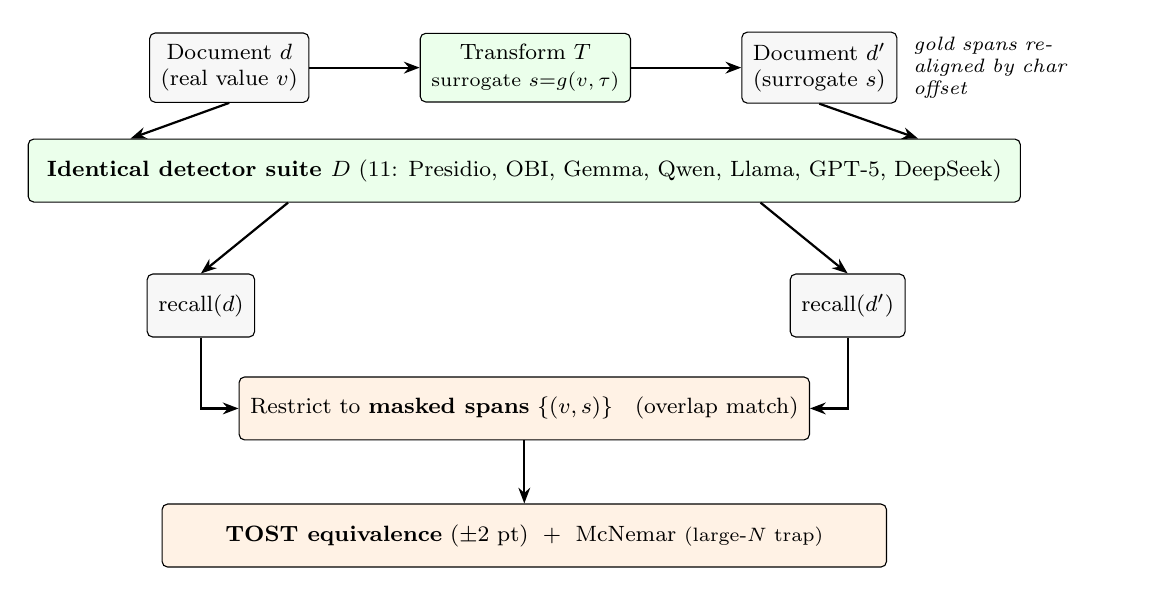
\begin{tikzpicture}[
  >={Stealth[length=2mm]}, font=\footnotesize,
  box/.style={draw,rounded corners=2pt,align=center,inner sep=4pt,minimum height=8mm,fill=black!3},
  op/.style={draw,rounded corners=2pt,align=center,inner sep=4pt,minimum height=8mm,fill=green!8},
  res/.style={draw,rounded corners=2pt,align=center,inner sep=4pt,minimum height=8mm,fill=orange!10},
  ar/.style={->,thick}
]
% top row: original -> transform -> transformed
\node[box] (d) {Document $d$\\(real value $v$)};
\node[op,right=14mm of d] (T) {Transform $T$\\{\scriptsize surrogate $s{=}g(v,\tau)$}};
\node[box,right=14mm of T] (dp) {Document $d'$\\(surrogate $s$)};
\draw[ar] (d) -- (T); \draw[ar] (T) -- (dp);
% detector suite spanning
\node[op,below=9mm of $(d)!0.5!(dp)$,minimum width=12.6cm] (det)
  {\textbf{Identical detector suite $D$} (11: Presidio, OBI, Gemma, Qwen, Llama, GPT-5, DeepSeek)};
\draw[ar] (d.south) -- ([xshift=-5cm]det.north);
\draw[ar] (dp.south) -- ([xshift=5cm]det.north);
% recalls
\node[box,below=9mm of det.south west,anchor=north,xshift=2.2cm] (ro) {recall$(d)$};
\node[box,below=9mm of det.south east,anchor=north,xshift=-2.2cm] (rt) {recall$(d')$};
\draw[ar] ([xshift=-3cm]det.south) -- (ro.north);
\draw[ar] ([xshift=3cm]det.south) -- (rt.north);
% restrict to masked spans
\node[res,below=9mm of $(ro)!0.5!(rt)$,minimum width=6.5cm] (mask)
  {Restrict to \textbf{masked spans} $\{(v,s)\}$ \; (overlap match)};
\draw[ar] (ro.south) |- (mask.west);
\draw[ar] (rt.south) |- (mask.east);
% tost
\node[res,below=8mm of mask,minimum width=9.2cm] (tost)
  {\textbf{TOST equivalence} ($\pm2$ pt) \;+\; McNemar {\scriptsize(large-$N$ trap)}};
\draw[ar] (mask) -- (tost);
% side annotations
\node[align=left,font=\scriptsize\itshape,right=1mm of dp,text width=2.5cm] {gold spans re-aligned by char offset};
\end{tikzpicture}
\caption{The paired evaluation protocol. Each document is scored in \emph{both} conditions ($d$, $d'$) by the identical 11-detector suite, so any per-span change is attributable to the substitution. Utility is measured \emph{only on masked spans}, and the paired recall difference is assessed with an equivalence test (TOST) rather than a significance test (\S\ref{sec:protocol}).}
\label{fig:protocol}
\end{figure*}

\section{Evaluation Protocol}\label{sec:protocol}
Figure~\ref{fig:protocol} summarizes the protocol. \textbf{Paired multi-detector design.} Each document is scored in two conditions---original $d$ and transformed $d'$---by the \emph{identical} detector suite $D$ ($|D|=11$). Because the only change between conditions is the substitution, any per-span change in detection is attributable to the substitution, not to the detector or the document.

\textbf{Metrics.} We report span-level P/R/F1 under three matching modes---\emph{exact} (start+end+type), \emph{type} (type+boundary), \emph{overlap} (any character overlap+type)---and \emph{leakage}~$=1-\text{recall}$, the HIPAA-critical quantity. The headline utility metric is \emph{recall retention on masked spans}~$=\text{recall}(d')/\text{recall}(d)$ restricted to $\{(v,s)\}$, under overlap matching (so pure boundary jitter from length changes, ``Anna~S.''$\rightarrow$``Maria~S.'', is not charged as a miss).

\textbf{Equivalence testing.} For pooled masked-span recall we run TOST with margin $\Delta=2$ points: we reject non-equivalence iff the 90\% CI of the recall difference lies entirely within $[-2,+2]$. We also report McNemar's test to illustrate the large-$N$ trap. We sweep $\Delta\in\{1,2,3\}$.

\textbf{Error attribution.} For the lost population (found on $d$, missed on $d'$) we hand-code each span into a small failure typology (\S\ref{sec:error}) and check length-preservation to separate boundary artifacts from genuine misses.

\section{Experimental Design}\label{sec:design}
\textbf{Detector panel~$D$.} Eleven detectors, three families: \emph{rule/statistical}---Microsoft Presidio, OBI \tp{deid\_roberta}; \emph{open LLMs (local)}---Gemma~4~31B, Gemma~4~E4B, Qwen~3.5-\{4B,\,9B,\,35B-A3B\}, Llama~3.1-8B, Llama~3.3-70B, DeepSeek~V2-Lite; \emph{frontier API}---OpenAI GPT-5. The panel is deliberately heterogeneous: if the equivalence result held only for one architecture it would be a model artifact, not a property of the transform.

\textbf{Benchmarks} (7; 250 docs each, 1{,}750 total). ASQ-PHI (English clinical queries), MEDDOCAN (Spanish clinical), MultiCoNER~v2 (multilingual NER)~\citep{fetahu2023multiconer}, and PII-Masking-300k~\citep{ai4privacy2023} in English, Dutch, French, German. Together: 7 languages, clinical and general-PII text, free-form and structured (JSON) formats. The transform under test is Custodian Guardian Layer \tp{transform} mode (top-1 surrogate, \tp{pii\_entities=ALL}).

\textbf{Comparison conditions.} The core study answers ``does \emph{this} transform preserve detectability.'' Three contrasts isolate \emph{why} and \emph{how generally}:
\begin{itemize}\itemsep2pt
\item \textbf{C1---Redaction upper-bound.} Replace each masked value with \tp{*****} (no surrogate signal) and re-detect; the transform$-$redact gap quantifies what structure preservation buys.
\item \textbf{C2---Open-source surrogate baseline.} Replace the commercial generator with an open one (Faker~\citep{faker}) on the \emph{same} masked spans; tests whether the result is generic to substitution or tool-specific, and makes the pipeline reproducible.
\item \textbf{C3---Per-benchmark equivalence.} Run TOST within each benchmark, sweeping $\Delta$, to check the pooled claim is not an averaging artifact.
\end{itemize}
The core paired study, the equivalence analysis (pooled and per-benchmark), the redaction floor, the open-surrogate baseline, and the error typology are complete; C1/C2 are currently demonstrated with the CPU detector (Presidio), with a full-panel extension noted as the next strengthening step.

\section{Results}\label{sec:results}
\textbf{Detectability is statistically unchanged.} Restricting to the 56{,}174 masked spans and pooling all 11 detectors, recall moves $76.2\%\rightarrow75.0\%$ ($-1.2$ pts; 95\% CI $[-1.5,-1.0]$). The TOST equivalence test ($\Delta=2$) rejects non-equivalence at $p\approx1\times10^{-8}$: the change is provably bounded within $\pm2$ points of zero. Ranking is preserved; the flagship Llama~3.3-70B is essentially unchanged ($\Delta$F1~$+0.003$). The same contingency is ``significant'' under McNemar's test---a direct demonstration of the large-$N$ trap.

\textbf{Recall retention on masked spans (overlap).} When the transform masks a span, detectors still find the surrogate 93--100\% of the time (Table~\ref{tab:ret}); the $\sim$3-point exact-boundary drop is a length-jitter artifact that vanishes under overlap matching.

\begin{table}[t]\centering\small
\begin{tabular}{lrr}
\toprule
System & Exact & Overlap\\
\midrule
Gemma 4 31B & 93.1 & \textbf{99.8}\\
Qwen 3.5-9B & 92.0 & \textbf{100.0}\\
Qwen 3.5-35B-A3B & 90.0 & \textbf{98.4}\\
Llama 3.3-70B & 91.4 & \textbf{98.3}\\
GPT-5 & 91.9 & \textbf{98.3}\\
Gemma 4 E4B & 88.9 & \textbf{98.2}\\
Qwen 3.5-4B & 84.7 & \textbf{98.0}\\
Presidio & 91.3 & \textbf{97.4}\\
DeepSeek V2-Lite & 87.7 & \textbf{92.8}\\
\bottomrule
\end{tabular}
\caption{Recall retention on masked spans (\%), transformed$\div$original.}\label{tab:ret}
\end{table}

\textbf{Per-benchmark equivalence (C3).} Table~\ref{tab:c3} (57{,}112 masked spans, via \tp{scripts/analyze\_equivalence.py}) shows the pooled equivalence is \emph{not uniform}: four benchmarks are equivalent within $\pm2$ points; MEDDOCAN and PII-nl require $\pm3$ (both dense, identifier-heavy, non-English---where surrogate generation is hardest, \S\ref{sec:error}); MultiCoNER has too few masked spans (220) to test. The honest claim: \emph{detectability is equivalent within $\pm2$ points on average and on clean text, and within $\pm3$ on the hardest identifier-dense text}---the residual is concentrated and attributable, not diffuse degradation.

\begin{table}[t]\centering\small
\begin{tabular}{lrrrl}
\toprule
Benchmark & Masked & O$\rightarrow$T & McN.\ $\chi^2$ & Margin\\
\midrule
ASQ-PHI & 5{,}427 & 91.9$\rightarrow$91.1 & 8.0 & $\pm2$\,\checkmark\\
MEDDOCAN & 31{,}978 & 73.4$\rightarrow$71.5 & 92.4 & $\pm3$\,\checkmark\\
MultiCoNER & 220 & 71.8$\rightarrow$71.4 & 0.0 & underpow.\\
PII en & 5{,}181 & 76.0$\rightarrow$75.1 & 4.0 & $\pm2$\,\checkmark\\
PII nl & 3{,}757 & 78.2$\rightarrow$76.3 & 13.1 & $\pm3$\,\checkmark\\
PII fr & 5{,}984 & 75.2$\rightarrow$75.9 & 3.5 & $\pm2$\,\checkmark\\
PII de & 4{,}565 & 76.3$\rightarrow$76.5 & 0.4 & $\pm2$\,\checkmark\\
\midrule
\textbf{Pooled} & \textbf{57{,}112} & \textbf{76.1$\rightarrow$74.9} & \textbf{82.1} & $\pm2$\,\checkmark\\
\bottomrule
\end{tabular}
\caption{Per-benchmark equivalence. O$\rightarrow$T = masked-span recall, original$\rightarrow$transform (\%). Pooled TOST $\Delta{=}2$: $p{=}3{\times}10^{-9}$.}\label{tab:c3}
\end{table}

\textbf{Redaction floor (C1).} Replacing masked values with \tp{*****} and re-detecting with Presidio (Table~\ref{tab:c1}): transform recall tracks the \emph{original} within a few points, while redaction collapses to $\approx$0--4\% (the residual is spurious overlap on the \tp{*} run). Structure-preserving substitution preserves essentially the entire detectability that redaction destroys.

\begin{table}[t]\centering\small
\begin{tabular}{lrrrr}
\toprule
Benchmark & Masked & Orig. & Transf. & Redact\\
\midrule
ASQ-PHI & 531 & 94.5 & 95.7 & \textbf{0.0}\\
MEDDOCAN & 2{,}925 & 75.4 & 72.9 & \textbf{0.0}\\
PII en & 471 & 75.6 & 73.5 & \textbf{1.9}\\
PII nl & 373 & 83.6 & 77.7 & \textbf{3.8}\\
PII fr & 544 & 61.4 & 59.9 & \textbf{2.2}\\
PII de & 415 & 56.1 & 58.3 & \textbf{0.0}\\
\bottomrule
\end{tabular}
\caption{C1 redaction floor: Presidio masked-span recall (\%).}\label{tab:c1}
\end{table}

\textbf{Open-surrogate baseline (C2).} Replacing the commercial generator with Faker on the same masked spans (Table~\ref{tab:c2}) yields two findings. \emph{Generality}: an open substitutor preserves masked-span recall at least as well as the original---detectability preservation is a property of well-formed same-type substitution, not one vendor, and reproduces without proprietary access. \emph{The residual is generator quality}: Faker, emitting clean canonical values, \emph{exceeds} the commercial transform by 18--20 points on the hard non-English benchmarks, precisely where the commercial surrogates truncate or garble (\S\ref{sec:error}).

\begin{table}[t]\centering\small
\begin{tabular}{lrrrr}
\toprule
Benchmark & Masked & Orig. & Custodian & Faker\\
\midrule
ASQ-PHI & 531 & 94.5 & 95.7 & \textbf{97.7}\\
MEDDOCAN & 2{,}925 & 75.4 & 72.9 & \textbf{79.7}\\
PII en & 471 & 75.6 & 73.5 & \textbf{89.2}\\
PII nl & 373 & 83.6 & 77.7 & \textbf{93.0}\\
PII fr & 544 & 61.4 & 59.9 & \textbf{78.5}\\
PII de & 415 & 56.1 & 58.3 & \textbf{78.1}\\
\bottomrule
\end{tabular}
\caption{C2 open-surrogate baseline: Presidio masked-span recall (\%). Detector-independent argument; Presidio-only demonstration.}\label{tab:c2}
\end{table}

\textbf{Leakage} barely moves ($+1.7$ to $+4.1$ pts across systems), so surrogates are not systematically easier to miss than the PHI they replace.

\section{Error Analysis}\label{sec:error}
\textbf{The lost population.} Pooled across detectors and masked spans: 39{,}550 spans found in both conditions; 3{,}261 lost. Critically, 51\% of lost spans are the \emph{same length} as the original---not a boundary effect. By type: LOCATION 28\%, NAME 23\%, DATE/AGE 22\%, ID/contact 20\%.

\textbf{Three failure modes---all generator-side.}
(1)~\emph{Malformed/truncated surrogates} (largest cause): \tp{Chicago}\arr\tp{Illino}, \tp{El~Paso}\arr\tp{El}, \tp{Ciudad de la Habana}\arr\tp{Cuidad de la Havana}. The fragment no longer matches the lexical pattern detectors learned for real names/places; this is why loss is highest on MEDDOCAN and lowest on clean English ASQ-PHI.
(2)~\emph{Loss of salience}: a canonical entity replaced by an obscure one (\tp{Cedars-Sinai}\arr\tp{Vidant}); detectors partly rely on pre-training familiarity, so swapping a famous value for a rare one removes the prior. Inherent to any value substitution; mainly costs weaker detectors.
(3)~\emph{\tp{x}-masking of IDs/emails}: \tp{nachorutor@\dots}\arr\tp{nxxxxxxxxx@\dots}. The \tp{x} run preserves format but breaks the realistic-token pattern. This case is \emph{privacy-positive}---the original value is destroyed---even though it counts against recall.

\textbf{Implication.} Detectors are not getting worse at PHI; the small recall gap is driven by surrogate-generation quality (truncation, garbling, salience, \tp{x}-masking). C2 confirms this directly: an open generator emitting clean canonical values \emph{exceeds} the commercial transform by 18--20 points on exactly the hard non-English benchmarks where its surrogates truncate---so the residual tracks generator quality, not the act of substitution.

\section{Discussion}
\textbf{What the evidence supports.} Structure-preserving substitution does not hide well-formed PHI from downstream detection. Because the effect is equivalence-bounded within $\pm2$ points and ranking-preserving across a heterogeneous 11-detector panel, a transform of this quality can be safely inserted ahead of detection/analytics pipelines built for real clinical text. \textbf{Generality (C2).} Faker preserves masked-span recall at least as well as the original across all six benchmarks, so $\pm2$ points is a property of well-formed substitution, not one vendor; where the commercial generator trails, a cleaner generator closes the gap, locating the residual squarely in generation quality. \textbf{A reusable protocol.} The paired masked-span design and the TOST margin are not specific to one vendor or language---a template for auditing any structure-preserving privacy transform.

\section{Ethics and Data Statement}
All benchmarks are public or synthetic (ASQ-PHI synthetic; MEDDOCAN released for a shared task; PII-Masking-300k synthetic; MultiCoNER~v2 public). \textbf{No real patient data is used.} We release the 250-document subsets and scoring code with license notes. \textbf{Dual-use.} A utility-preserving de-identifier could in principle launder identifiable data into a fluent form; our masked-span/leakage reporting and the privacy-positive framing of \tp{x}-masking keep the privacy accounting explicit. \textbf{Conflict of interest.} The commercial transform (Custodian Guardian Layer) is developed by Custodian Labs, with which one or more authors are affiliated; this work was conducted with Custodian Labs' support. To limit bias we (i)~frame the contribution as a reusable protocol, (ii)~include open-source baselines so results are reproducible without proprietary access, and (iii)~report leakage and coverage alongside utility.

\section{Limitations}
Coverage is reported but not the focus; a transform can preserve utility on what it masks while under-masking (the axes are independent by design). 250~docs/benchmark bounds per-benchmark power (though the pooled masked-span $N$ is large). C1/C2 are currently demonstrated with a CPU detector (Presidio); a full 11-detector extension is future work. LLM detectors are prompt-sensitive; we fix one prompt per model (appendix).

\bibliographystyle{plainnat}
\bibliography{refs}

\end{document}
